\documentclass[french]{article}
\usepackage{graphicx}
\usepackage{babel}
\usepackage[a4paper, total={6in, 10in}]{geometry}
\usepackage{graphicx}
\usepackage{listings}
\usepackage{color}
\usepackage{pdfpages}
\usepackage{caption}

\usepackage[svgnames]{xcolor} % Required for colour specification
\usepackage[utf8]{inputenc} % Required for inputting international characters
\usepackage[T1]{fontenc} % Output font encoding for international characters
\usepackage{fouriernc} % Use the New Century Schoolbook font

\DeclareGraphicsExtensions{.pdf,.png,.jpg}
% listings color configuration to display beautifuuul code
\definecolor{Monokaigreen}{rgb}{0.42,0.72,0.18}
\definecolor{Monokaimagenta}{rgb}{0.86,0.08,0.24}
\definecolor{Monokaiblue}{rgb}{0.40,0.85,0.94}
\definecolor{Monokaibg}{rgb}{0.15,0.16,0.13}
\definecolor{splashedwhite}{rgb}{1.0, 0.99, 1.0}
\definecolor{richelectricblue}{rgb}{0.03, 0.57, 0.82}
\definecolor{pinegreen}{rgb}{0.0, 0.47, 0.44}
\definecolor{ivory}{rgb}{1.0, 1.0, 0.94}
\definecolor{ghostwhite}{rgb}{0.97, 0.97, 1.0}
\definecolor{floralwhite}{rgb}{1.0, 0.98, 0.94}
\definecolor{gray}{rgb}{0.5,0.5,0.5}

 
\definecolor{codegreen}{rgb}{0,0.6,0}
\definecolor{codegray}{rgb}{0.5,0.5,0.5}
\definecolor{codepurple}{rgb}{0.58,0,0.82}
\definecolor{backcolour}{rgb}{0.95,0.95,0.92}

\lstdefinestyle{code_style}{
    backgroundcolor=\color{backcolour},   
    commentstyle=\color{codegreen},
    keywordstyle=\color{magenta},
    numberstyle=\tiny\color{codegray},
    stringstyle=\color{codepurple},
    basicstyle=\footnotesize,
    breakatwhitespace=false,         
    breaklines=true,                 
    captionpos=b,                    
    keepspaces=true,                 
    numbers=left,                    
    numbersep=4pt,                  
    showspaces=false,                
    showstringspaces=false,
    showtabs=false,                  
    tabsize=2
}

\lstset{style=code_style}
 

\makeatletter
%same as \subsubsection but level 4
\renewcommand\paragraph{\@startsection{paragraph}{4}{\z@}%
                                     {-3.25ex\@plus -1ex \@minus -.2ex}%
                                     {1.5ex \@plus .2ex}%
                                     {\normalfont\normalsize\bfseries}}
% number \paragraph
\setcounter{secnumdepth}{4}

\lstset{frame=shadowbox,
	language=Java,
	aboveskip=3mm,
	belowskip=3mm,
	showstringspaces=false,
	columns=flexible,
	basicstyle={\small\ttfamily},
	numbers=left,
	numberstyle=\tiny\color{gray},
	keywordstyle=\color{Monokaibg}\bfseries,
	commentstyle=\color{pinegreen},
	stringstyle=\color{Monokaigreen},
	breaklines=true,
	breakatwhitespace=false,
	tabsize=3,
	captionpos=b,                    % sets the caption-position to bottom
	frame=single,
	rulecolor=\color{gray},
}

\title{Sections and Chapitres}
\author{Quentin Gigon}
\date{ }

\begin{document}

\begin{titlepage} % Suppresses headers and footers on the title page
	
	\centering % Centre everything on the title page
	
	%------------------------------------------------
	%	Top rules
	%------------------------------------------------
	
	\rule{\textwidth}{1pt} % Thick horizontal rule
	
	\vspace{2pt}\vspace{-\baselineskip} % Whitespace between rules
	
	\rule{\textwidth}{0.4pt} % Thin horizontal rule
	
	\vspace{0.1\textheight} % Whitespace between the top rules and title
	
	%------------------------------------------------
	%	Title
	%------------------------------------------------
	
	\textcolor{Red}{ % Red font color
		{\Huge TB}\\[0.5\baselineskip] % Title line 1
	}
	
	\vspace{0.025\textheight} % Whitespace between the title and short horizontal rule
	
	\rule{0.3\textwidth}{0.4pt} % Short horizontal rule under the title
	
	\vspace{0.1\textheight} % Whitespace between the thin horizontal rule and the author name
	
	%------------------------------------------------
	%	Author
	%------------------------------------------------
	
	{\Large \textsc{Quentin Gigon}} % Author name
	
	\vfill % Whitespace between the author name and publisher
	
	%------------------------------------------------
	%	Publisher
	%------------------------------------------------
	
	{\large\textsc{HEIG-VD}} % Publisher
	
	\vspace{0.1\textheight} % Whitespace under the publisher text
	
	%------------------------------------------------
	%	Bottom rules
	%------------------------------------------------
	
	\rule{\textwidth}{0.4pt} % Thin horizontal rule
	
	\vspace{2pt}\vspace{-\baselineskip} % Whitespace between rules
	
	\rule{\textwidth}{1pt} % Thick horizontal rule
	
\end{titlepage}

\maketitle

\tableofcontents
\newpage

\section{Introduction au projet}
Le but de ce travail est de pouvoir visualiser et gérer l'affichage de divers flux d'information sur les écrans des différents campus de la HEIG, comme par exemple les horaires de cours, les news de la RTS, les réservations de salles, etc, à travers une interface web.

\section{Cahier des charges}
A remettre à jour!!

\subsection{Contraintes et besoins}
Les besoins principaux de cette application sont les suivants:
\begin{itemize}
	\item Gestion de l'affichage de flux d'information sur des écrans dans la HEIG-VD (smartTV ou ordinateur) par une interface web.
	\item Protocole concis de communication entre les écrans et le serveur limitant les échanges.
	\item Affichage de flux "controlés" (générés par l'application, par exemple un flux RSS) et "non-controlés" (flux de la RTS, horaires des cours, etc).
	\item Un Schedule qui s'occupe de changer les flux affichés selon un horaire prédéfini.
	\item Une modélisation générique des flux et une factorisation de ceux venant de sources externes afin de pouvoir les envoyer de la même manière aux écrans
	\item La possibilité de diffuser plusieurs types de médias (images, vidéos, etc)
	\item La possibilité de passer outre le Schedule et d'afficher un flux voulu (annonce importante, etc) avec reprise de l'exécution prévue par la suite. \newline
\end{itemize}


\textbf{Quelques précisions:}
Un Schedule est un "horaire" qui gère le changement de flux selon un ordre choisi par l'utilisateur. Il n'y aura pas qu'un seul Schedule mais plutôt la possibilité d'en créer plusieurs qui soient assignables à un écran ou groupe d'écrans.
\newline


Les contraintes principales quand à elles sont les suivantes:
\begin{itemize}
	\item L'affichage des flux doit être fait dans un navigateur supportant le Javascript, HTLM5 et CSS3.
	\item Il doit y avoir une base de données qui enregistre les utilisateurs ainsi que les écrans.
	\item Il y a plusieurs types d'utilisateurs qui, selon leur emplacement (campus) et/ou leur niveau d'autorisation, peuvent modifier l'affichage des écrans.
	\item Le système doit être tolérant face aux panne, avec une reprise automatique.
	\item Le système doit disposer d'une interface simple et être utilisable par des gens du domaine et par des personnes non-initiées.
\end{itemize}


\subsection{Fonctionnalités}
Les fonctionnalités nécessaires et principales du programme sont divisées en plusieurs catégories:
\begin{itemize}
	\item \textbf{Frontend}
	\begin{enumerate}
		\item Interface de login et register sur le site (register dans le cadre du TB)
		\item Ecrans
		\begin{enumerate}
			\item Visualisation des écrans actifs et de leur emplacement sur le campus (une "carte" par site)
			\item Visualisation des informations d'un écran spécifique (et groupe d'écrans)
			\item Modification de la diffusion actuelle sur un écran/groupe d'écrans (flux "hors-runningSchedule", attribution à un Schedule, arrêt de la diffusion, ...)
		\end{enumerate}
		\item Flux
		\begin{enumerate}
			\item Opérations CRUD sur les flux (interface de création)
			\item Visualisation des flux utilisables par le système et infos sur leur contenu
		\end{enumerate}
		\item Schedules
		\begin{enumerate}
			\item Opérations CRUD sur les Schedules (interface de création)
			\item Visualisation des Schedules utilisables par le système et infos sur leur contenu et horaire
		\end{enumerate}
		\end{enumerate}
	\item \textbf{Backend - Play!}
	\begin{enumerate}
		\item Ecrans
		\begin{enumerate}
			\item Opérations CRUD sur les écrans
			\item Emission de token d'authentification pour la connexion des écrans
		\end{enumerate}
		\item Flux
		\begin{enumerate}
			\item Opérations CRUD sur les flux
			\item Diffusion de flux aux écrans selon un Schedule
			\item Diffusion de flux hors-runningSchedule (annonces, alertes, etc)
			\item Formatage et mise en page des flux externes (RTS ou autre)
		\end{enumerate}
		\item Schedules
		\begin{enumerate}
			\item Opérations CRUD sur les Schedules
			\item Assignation d'un Schedule à un écran/groupe d'écrans
		\end{enumerate}
		\item Utilisateurs
		 \begin{enumerate}
			\item Register 
			\item Login 
			\item Niveaux d'autorisation
		\end{enumerate}
	\end{enumerate}
	
	\item \textbf{Base de données}
	\begin{enumerate}
		\item Utilisateurs avec différents niveaux d'autorisations
		\item Ecrans, avec leurs caractéristiques et emplacement
		\item Flux utilisés par le système
		\item Schedules de flux \newline
	\end{enumerate}
\end{itemize}

Les fonctionnalités suivantes sont considérées comme secondaires et seront réalisées si le temps le permet:
\begin{itemize}
	\item \textbf{Frontend}
	\begin{enumerate}
		\item Modification en live du contenu d'un flux
	\end{enumerate}
	\item \textbf{Backend}
	\begin{enumerate}
		\item Monitoring de l'état des écrans (log du dernier échange avec l'écran)
		\item Schedul-ception (Schedule dans un Schedule)
	\end{enumerate}
\end{itemize}

\subsection{Echéancier}

Le travail sera divisé en 4 parties :
\begin{itemize}
	\item \textbf{Analyse et Modélisation} (2 semaines) \newline
	Analyse des contraintes et besoins du travail et modélisation d'un système parvenant à y répondre (schémas de DB, modélisation des flux, etc)
	\item \textbf{Architecture} (1 semaine) \newline
	Création d'une architecture de code permettant la réalisation d'un programme efficace, modulable et améliorable par la suite
	\item \textbf{Développement et Tests} (7 semaines) \newline
	Codage de l'application, en commençant par le serveur et en finissant avec le frontend.  
	Création de la base de données en parallèle.
	Tests unitaires et fonctionnels (60-70\% de coverage visé)
	\item \textbf{Rapport et Documentation} (3 semaines) \newline
	\end{itemize}
	
Total: env. 13 semaines à partir du 25.02 \newpage

\newpage
\section{Présentation des technologies utilisées}

\subsection{Framework Play!}
Play! est un framework web open-source qui suit le modèle MVC et qui permet d'écrire rapidement des application web en Java (ou en Scala). A la différence d'autre frameworks Java, Play! est \textit{stateless}, ce qui veut dire qu'il n'y a pas de session JavaEE créée à chaque connexion. 
Il fourni aussi à ses utilisateurs des frameworks de tests unitaires et fonctionnels, à savoir JUnit et Selenium.


\subsection{EventSource}
Les EventSource, ou Server-Sent Events (SSE), sont une technologie permettant à un navigateur internet de recevoir des mises à jour automatiques d'un serveur par une connexion HTTP persistante. L'API Javascript (\textit{Server-Sent Events EventSource API}) fut instaurée la première fois dans Opera en 2006 et a été normalisée dans le cadre de HTML5. \par
Les Events envoyés sont au format \textit{text/event-stream} et sont reçus par le navigateur sous la forme d'Event de type \textit{message} La connexion reste ouverte tant qu'elle n'a pas été fermée par le navigateur, et contrairement aux WebSockets, les SSE sont uni-directionnels et ne permettent donc pas aux clients de communiquer avec le serveur. 

\subsection{PostgreSQL}
PostgreSQL est un système de gestion de base de données relationnelle et open-source. La différence principale entre PostgreSQL et ses concurrents est la prise en charge de plus de types de donnée que les types traditionnels (entiers, caractères, ...).

\subsection{JPA}
La Java Persistence API (JPA) est une interface de programmation permettant aux utilisateurs de la plateforme Java (SE et EE) d'organiser facilement et clairement leurs données relationnelles. Elle utilise des annotations pour définir des "objet-métiers" qui serviront d'interface entre la base de données et l'application. \newline
JPA définit aussi le Java Persistence Query Language (JPQL), qui est utilisé pour créer les requêtes SQL dans le cadre de JPA. Les requêtes effectuées dans ce langage ressemblent beaucoup à du SQL classique, sauf que le JPQL fonctionne avec des entités (créées avec des annotations) plutôt que des tables de la base de données.

\subsection{JWT}
Un JSON Web Token est un standard ouvert permettant l'échange sécurisé de jetons d'accès entre plusieurs parties. Les jetons sont signés à l'aide d'une clé privée (très souvent le serveur) et fournis aux client qui doivent l'intégrer à leurs prochaines requêtes. Un jeton n'est pas associé à un utilisateur mais plutôt à un rôle (p.ex. administrateur) et à une durée de validité définie par le serveur également. Ils sont très souvent utilisés pour gérer des utilisateurs (login).

\subsection{HTML5}
HTML5 est la dernière version majeure du HTML (octobre 2014). Elle vient avec plein de nouveaux élément, comme la balise \textit{video}, qui permet d'insérer un contenu vidéo en streaming dans un fichier HTML, ou encore \textit{footer}, qui lui permet de facilement afficher du texte en bas de page.

\newpage
\section{Schéma de base de donnée}
Une des directives principales du projet était la représentation en tout temps de l'état actuel du programme en base de données. Le schéma a donc été pensé pour répondre à cette demande. Les limitations voulues pour les différents rôles des utilisateurs et pour les services de la HEIG (COM, Secrétariat, Baleinev, etc) sont toutes représentées en BD, comme par exemple un PhysicalScreen est relié à un site (ce qui limite les flux qu'il peut afficher) et il est également relié à une ou plusieurs Teams (autorise uniquement les membres de cette Team à interagir avec cet écran).
\newline TODO : explications du schéma une fois celui-ci définitif (ou presque).

	\begin{figure}[h]
		\centering
		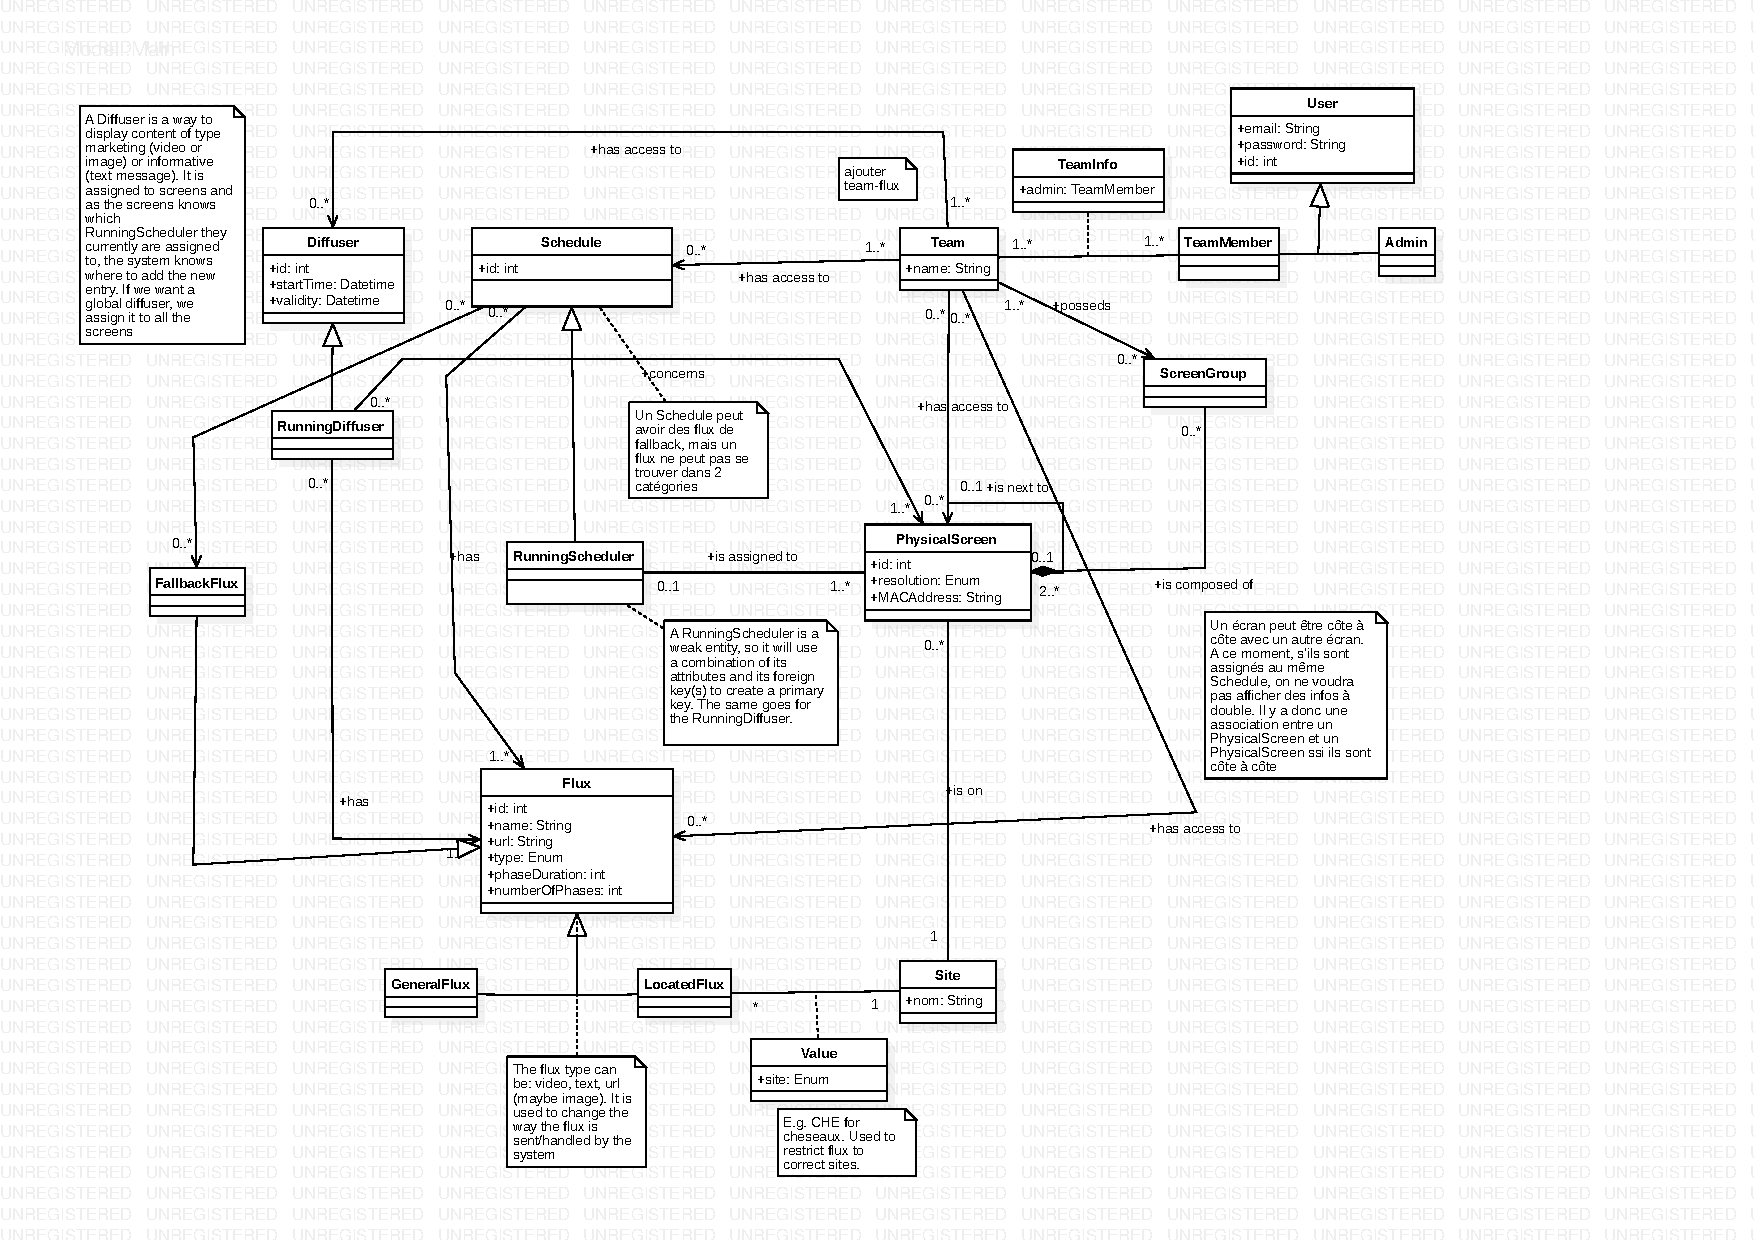
\includegraphics[scale=0.5]{db_schema}
		\caption{Schéma de base de données}
	\end{figure}

\newpage
\section{Analyse et Architecture}

Dans les chapitres suivants seront détaillés l'architecture du programme, ainsi que les différentes idées et versions qui ont été envisagées.

\subsection{Site}
Un site représente un emplacement physique de l'HEIG-VD, donc les sites de Cheseaux, St-Roch et Y-Park. Ils servent principalement à localiser les écrans et restreindre l'affichage de flux selon le lieu. 

\subsection{Team}
Pendant la phase d'analyse, il a été spécifié qu'un système d'équipe était nécessaire, afin de restreindre les fonctions du programme selon l'appartenance de l'utilisateur à telle ou telle équipe. Cela faisait également sens vu que le programme serait utilisé par les différents département de la HEIG-VD.\newline
Les \textbf{Teams} ont donc une place centrale dans l'architecture du programme dans le sens que les actions proposées à l'utilisateur utilisent uniquement les données accessibles par son équipe. Elle est composée de membres et de chefs d'équipe, qui sont les deux représentés par des \textbf{TeamMember}, et qui ont différents niveaux d'accès.

\subsection{Organisation des flux}

Un flux dans ce programme représente un contenu à afficher sur un écran. Ce contenu peut avoir des origines différentes, par exemple un flux externe à l'application comme le flux de la RTS ou un flux interne, comme les horaires des cours ou les réservations de salle. \newline
Lors de la phase d'analyse, il a été spécifié que le programme devrait pouvoir gérer au moins deux catégories de flux:
\begin{itemize}
	\item Des flux externes (p.ex. flux de la RTS)
	\item Des flux internes, avec la possibilité de les interroger pour savoir s'ils ont du contenu à afficher (réservation de salle, élection du CoRe) 
\end{itemize}

J'avais également proposé de fournir un template RSS permettant un ajout facile de nouveau flux RSS, mais cette fonctionnalité à été abandonnée par manque de temps.

En ce qui concerne leur diffusion, il fallait proposer un moyen d'organiser un horaire de flux ainsi que la possibilité d'envoyer immédiatement un flux sur un écran. Deux types d'objets ont été créés pour cela: des Schedules (horaires), qui représentent l'horaire d'une journée et des Diffusers, qui eux permettent d'ajouter une entrée sur l'horaire d'un ou plusieurs écrans. 

\subsubsection{Flux}

Un flux est caractérisé par un nom, type, une durée d'affichage et un contenu. Ce contenu est défini par le type du flux; un flux 'URL' contiendra une url, tandis un flux de type 'Image' contiendra l'adresse de l'image sur le serveur.

Ils sont regroupés en quatre types:
\begin{itemize}
	\item URL, ou type standard
	\item Vidéo
	\item Image
	\item Texte
\end{itemize}
Le traitement de ces flux par le système et la manière par-laquelle ils sont affichés sur les écrans changent selon leur type. Par exemple, un flux 'Image' sera rendu dans une balise <img>, tandis qu'un flux 'URL' le sera dans une "iframe".

De plus, il y a trois sortes de flux: des flux généraux, des flux localisés et des flux de fallback. Ces trois groupes sont a voir comme des sous-populations de flux: ils ont une référence vers un flux. \newline
Comme son nom l'indique, un flux général peut être diffusé partout. Un flux localisé est lui uniquement affichable sur le Site correspondant. On peut donc par exemple avoir un seul flux pour les horaires de cours et plusieurs flux localisés qui le référence, en fournissant selon le site où il est envoyé un paramètre de requête différent (-> http://heig.com/horaires?site=che). Cette information est stockée dans la base de donnée sous la forme d'une table intermédiaire entre Site et LocatedFlux. \newline
Et enfin un flux peut être un flux de fallback. Ces flux sont spécifiés à la création d'un Schedule et utilisés par celui-ci pour remplacer un flux programmé mais pour lequel le serveur ne détecte aucune données à afficher. Ces flux peuvent être généraux ou localisés. \newline \par

\subsubsection{Schedules}
Un Schedule représente un horaire de flux. Un Schedule n'est pas assigné à des écrans à sa création mais au moment de son activation pour permettre  une réutilisation plus facile des Schedules créés. Chaque chef d'équipe peut en créer qui seront utilisables par tous les membres de son équipe. \newline

La première version de cet horaire modélisait un cycle, où les flux choisis par l'utilisateur bouclaient à l'infini. Ce système a été utilisé avec succès pour de la recherche et des tests sur la faisabilité du programme mais fut vite obsolète quand il s'agissait d'avoir plus de contrôle sur l'horaire, par exemple définir une heure de début pour un flux donné. \newline
Il a donc fallu inventer un système permettant à la fois de créer un horaire à respecter pour les Schedules et de modifier cet horaire à la volée pour les Diffusers, tout en garantissant la cohérence du programme. 
	\newline
J'ai choisi de représenter une journée complète d'affichage par des blocs de 1 minute chacun. Cette plage d'affichage est bornée par une heure de départ (inclusive) et une heure de fin (exclusive) qui sont fixes, mais modifiables si besoin. A titre d'exemple, en prenant les valeurs que j'ai défini, soit de 8h à 22h, on obtient une plage horaire de 15h, ce qui est équivalent à 900 blocs. 
Si on regarde maintenant pas-à-pas la procédure de création puis d'activation d'un Schedule:

Quand un utilisateur crée un Schedule, il peut lui spécifier plusieurs choses:
\begin{itemize}
	\item Un nom (unique)
	\item Des flux avec heure de début (ScheduledFlux)
	\item Des flux sans heure de début 
	\item Des flux de fallback
	\item Garder l'ordre des flux ou non
\end{itemize}

Pour chaque flux avec une heure de début associée, une "entrée de calendrier", ou ScheduledFlux, est créée. Cette "entrée" contient des références vers le Flux et le Schedule concerné, ainsi que le numéro de son bloc de départ.\newline
Chaque flux sans heure de début est simplement ajouté au Schedule, pareil pour les flux de fallback. L'option de garder l'ordre des flux permet de garantir que les flux sans heure fixe seront affichés dans l'ordre dans lequel l'utilisateur les a rentré. Notre Schedule est maintenant créé, il ne reste plus qu'a l'activer.\newline

A l'activation d'un Schedule, on peut choisir parmi les écrans auxquels on a accès ceux qui seront concernés. Un objet RunningSchedule est créé, une entité temporaire qui existe uniquement tant que le Schedule reste actif. 
Cette entité est ensuite utilisée pour créer un "bloc-horaire", qui associe avec chaque bloc le flux correspondant (en regardant parmi les ScheduledFlux) ou une absence de flux. Un Runnable (RunningScheduleThread) est ensuite lancé avec cet horaire. La manière dont il choisit le prochain flux est détaillée dans la section correspondante.\newline 
Ce système permet de répondre à une autre demande du projet, la reprise de l'exécution des Schedules actifs lors du redémarrage du serveur ou après une maintenance. En donnant un moyen de faire correspondre une heure donnée avec un numéro de bloc, on peut très facilement reprendre l'exécution la où elle s'était arrêtée.


\subsubsection{Diffuser}
Un Diffuser est quand à lui utilisé pour diffuser un flux de catégorie marketing ou un message unique sur une quantité X d'écrans. Ils fonctionnent en changeant les Schedules actifs associés à ces écrans pour ajouter le flux souhaité dans leur horaire. Ce système offre plusieurs possibilités de customisation, comme spécifier la durée du flux ou limiter dans le temps la diffusion de ce flux (p.ex. modifier les Schedules actifs seulement pendant une semaine et revenir à l'état de base après). Au moment de l'ajout du flux dans le Schedule, des vérifications sont faites pour garantir un bon fonctionnement par la suite (on peut imaginer que l'heure choisie pour le nouveau flux soit déjà prise, il faudra alors avertir l'utilisateur qu'il ne peut effectuer cette action ou alors autoriser l'action mais adapter l'heure de démarrage du nouveau flux pour ce Schedule). \newline
Comme pour les Schedules, un Diffuser actif est un RunningDiffuser, lui aussi une entité temporaire qui reste active selon la validité spécifiée à sa création. Un fois que le RunningDiffuser est arrivé en fin de vie, le flux qu'il avait rajouté dans les RunningSchedules est enlevé. 


\subsection{Ecrans}

Lors de mes discussions avec mon mentor, il a été assez vite recommandé et conseillé que j'utilise des Eventsources (voir doc) pour envoyer les ordres d'affichages aux écrans. Les sections suivantes résument et décrivent leur utilisation dans ce programme.

\subsubsection{Affichage}
Pour l'affichage des flux sur les écrans, les technologies autorisées étaient le HTML5, CSS3 et Javascript pur (sans frameworks). La demande initiale était de pouvoir afficher le contenu associé à une URL grâce aux iframes. Il fallait donc un moyen pour les écrans de recevoir une URL sous forme texte. En partant de ce constat, j'ai remarqué que si un Event contenait une URL en texte, il pouvait contenir d'autres données. J'ai donc proposé d'implémenter des flux de type image et texte. \newline
Les écrans sont donc capable de déterminer le type du flux reçu et de l'afficher de la manière adéquate. Les différents moyens utilisés l'affichage en question sont décrit dans la section Réalisation.

\subsubsection{Events}
Un des problèmes à résoudre était la question d'envoyer les bons Events aux bons écrans.
 Il y avait deux manières principales de faire, soit envoyer tous les Events à tous les écrans avec la liste des écrans concernés, soit générer dynamiquement des endpoints pour chaque Schedule. Pour des raisons de simplicité et parce que le nombre d'écrans restera raisonnable, la première possibilité a été choisie. \newline
Les Events générés par les Schedules sont donc envoyés à tous les écrans s'étant connecté auprès du serveur. Chaque Event contient les adresses MAC des écrans concernés et c'est à l'écran de vérifier s'il est concerné par l'Event qu'il vient de recevoir.\newline
Un Event est construit de la manière suivante: il contient son type, ses "données" (url ou texte) et les écrans concernés. Ci-dessous un exemple pour chaque type:
\begin{itemize}
	\item URL:\begin{verbatim}
					url?https://heig-vd.ch|mac_address1,mac_address2
			  \end{verbatim}
	\item Image: \begin{verbatim}
					image?/assets/image1|mac_address2, mac_address3
			  \end{verbatim}
	\item Video: \begin{verbatim}
					video?https://www.youtube.com/embed/dQw4w9WgXcQ|mac_address1, mac_address3
			  \end{verbatim}
	\item Texte: \begin{verbatim}
					text?Hello World|mac_address2
			  \end{verbatim}
\end{itemize}


\subsubsection{Authentification}
Un écran ne peut recevoir d'Event qu'une fois authentifié, pour des raisons évidentes de sécurité. Il fallait donc trouver un moyen d'identifier de manière unique chaque écran. La première piste envisagée fut d'utiliser les hostnames des écrans car cette information était facilement récupérable en Java, et spécialement avec Play. Mais en raison de l'architecture réseau de la HEIG et de la volonté d'intégrer le protocole WakeOnLan au programme, il a été décidé d'utiliser les adresses MAC à la place. \newline 
La difficulté inhérente à ceci était de récupérer ces adresses depuis Java. Pour remédier à ce problème et en même temps fournir une couche de sécurité au niveau des écrans, il a été choisi que lors de l'ajout d'un écran au système, son adresse MAC devrait être précisée. \newline

L'accès des écrans serveur se fait en deux étapes. Il faut d'abord que l'écran se connecte à la route d'authentification des écrans, tout en spécifiant 
comme paramètre de requête son adresse MAC. Exemple:
\begin{verbatim}
	http://server/screens/auth?mac=1234
\end{verbatim}

Là, si l'adresse est inconnue par le serveur, il nous renvoie un code permettant l'ajout de l'écran dans le système depuis le site web. Si l'adresse est connue, il ajoute ajoute dans les cookies l'adresse MAC de l'écran ainsi que sa résolutions (utile pour la gestion de l'affichage), passe l'écran comme actif et le redirige sur le endpoint

\subsubsection{Groupe d'écrans}
Les groupes d'écrans sont créés par des chefs d'équipe et donc uniquement disponible à l'intérieur d'une Team (on pourrait aussi imaginer des groupes communs à toutes les Teams). Ils servent à regrouper les écrans selon leur utilité, pour faciliter leur assignement à un Schedule. Par exemple, un groupe d'écran possible serait celui des écrans du hall de Cheseaux. \newline
Un écran peut faire partie de plusieurs groupes, mais comme précisé plus haut, il ne peut être associé qu'a un RunningSchedule à la fois. Il y aura donc des vérifications qui seront faites au moment d'activer un Schedule sur un groupe d'écran pour empêcher ceci.

\newpage

		
\section{Protocole de communication écran-serveur}
TODO: refaire les images.\newline
	Le protocole ci-dessous explique et détaille la communication entre les écrans et le serveur, ainsi que les erreurs potentielles et leur prise en charge. 
	
\subsection{Ecran inconnu du serveur}
	Dans ce cas de figure, l'écran n'a pas encore été ajouté au système par l'administrateur, et donc le serveur ne reconnait pas son adresse MAC lors de la connexion. A ce moment, il lui renvoie une page HTML qui affiche un code (propre à chaque écran) a utiliser pour introduire l'écran dans le système.
	
		\begin{figure}[hbt!]
			\centering
			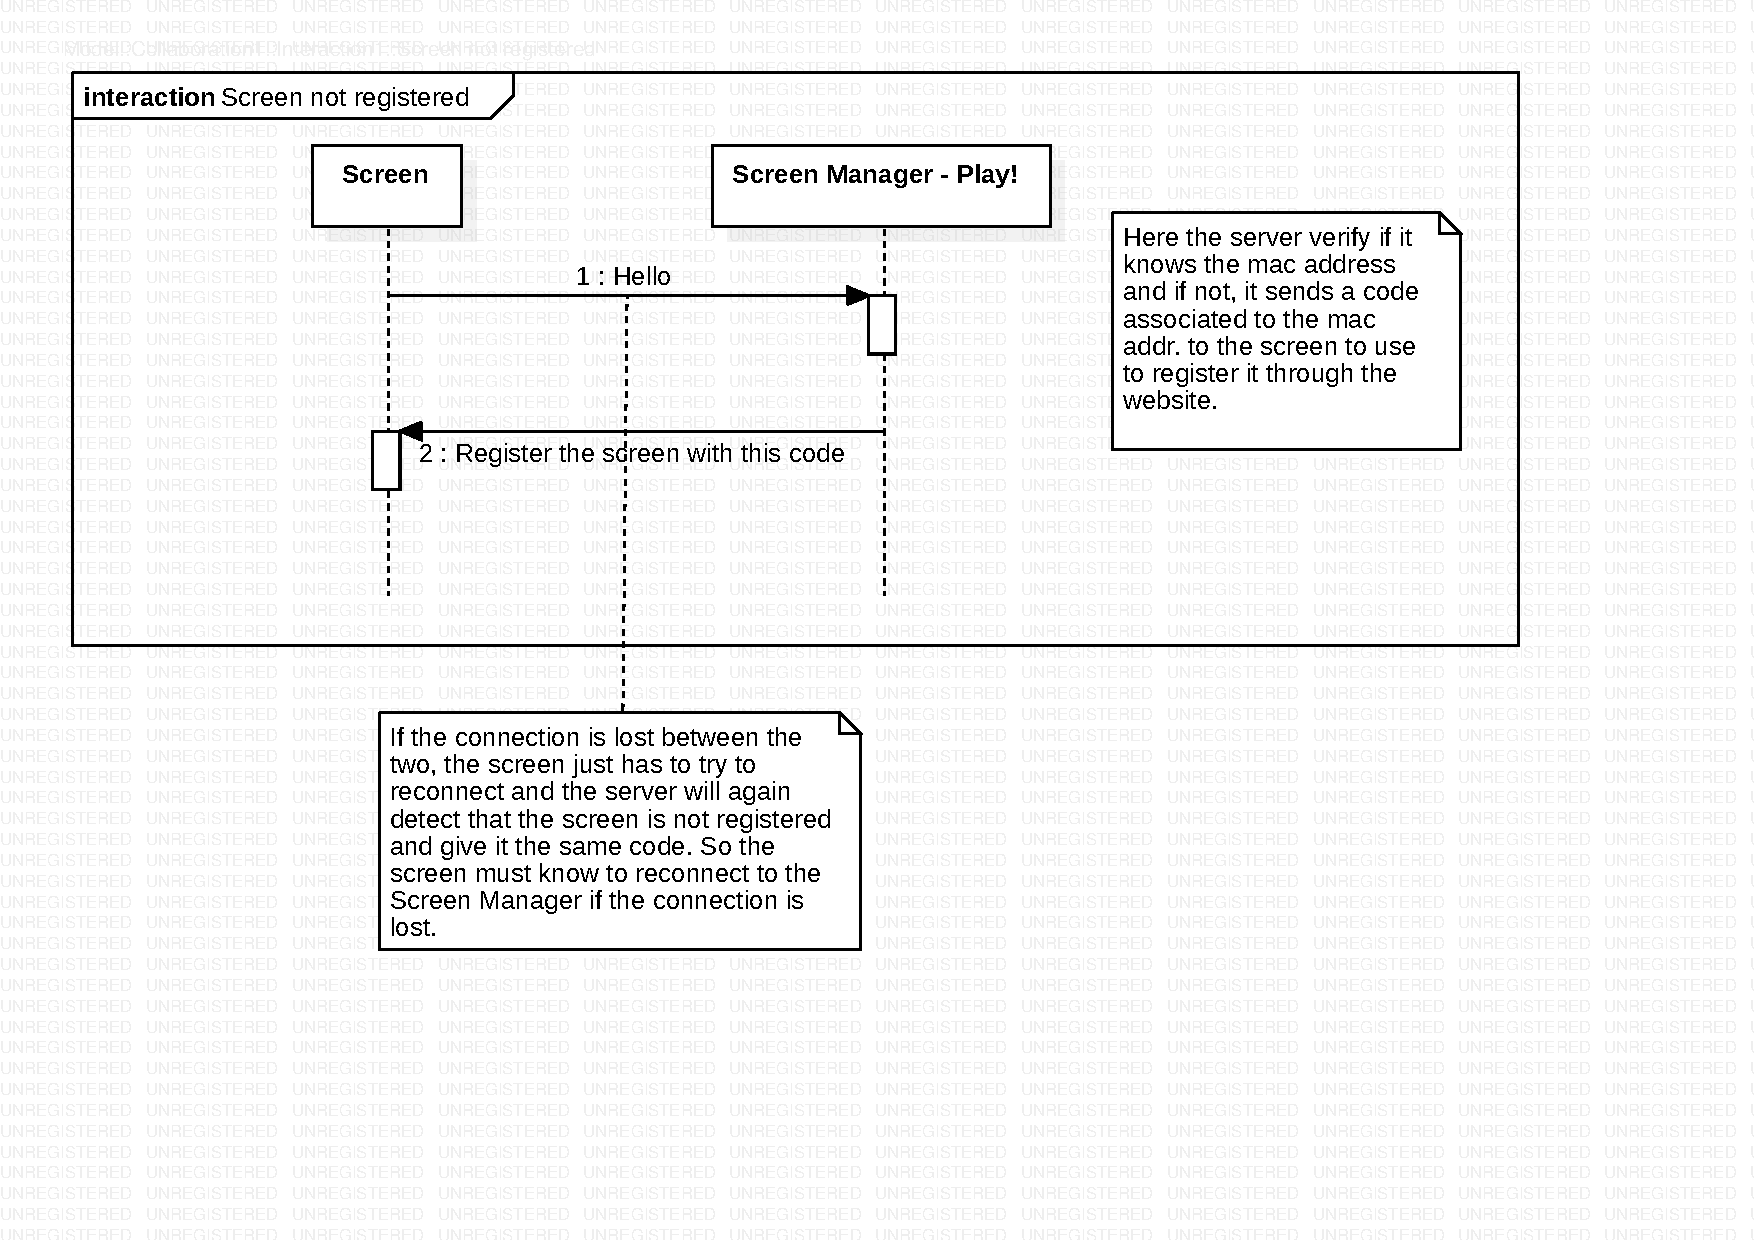
\includegraphics[page={1}, scale=0.5]{protocol_v2}
			\caption{Ecran inconnu}
		\end{figure}
	
	Le fait que l'écran perde sa connexion Internet pendant cet échange ne devrait poser aucun problème car le code sera simplement ré-envoyé à l'écran lors de sa prochaine connexion (en effet l'adresse MAC sera toujours inconnue du serveur). \newpage
	
\subsection{Ecran connu du serveur}
	La figure suivante décris le cas idéal, où l'écran est connu par le serveur et il n'y a pas de perte de connexion.
	\begin{figure}[h!]
		\centering
		\includegraphics[page={3}, scale=0.5]{protocol_v2}
		\caption{Ecran connu}
	\end{figure}			
	L'adresse MAC de l'écran est cette fois connue par le serveur, donc il marque l'écran comme actif (logged in) et vérifie si l'écran est associé avec un RunningSchedule. Si c'est le cas, il ajoute son adresse MAC dans la liste des écrans concernés par ce Schedule et le redirige vers le endpoint d'envoi d'Events. Dans le cas contraire, l'écran affiche simplement un message générique (p.ex. "Ecran non-assigné..."). \newpage
	
\subsection{Ecran connu - erreurs de connexion}
	Ici sont listées les actions effectuées par le serveur ou le client en cas d'erreurs lors la phase d'authentification.
	\begin{figure}[h!]
		\centering
		\includegraphics[page={2}, scale=0.5]{protocol_v2}
		\caption{Ecran connu - erreurs}
	\end{figure}
	
			
	Comme précédemment, le fait qu'un écran perde sa connexion au serveur lorsqu'il essaie de s'authentifier ne devrait pas poser de problèmes, car il lui suffit de ré-essayer. \newline
	Par contre, si l'écran perd sa connexion une fois qu'il s'est identifié auprès du serveur, il faudra le retirer de la liste des écrans concernés par son RunningSchedule jusqu'à ce qu'il se re-connecte. \newpage
	
	
\section{Réalisation technique}

\subsection{Organisation des flux}

Cette section se concentre sur la manière dont la diffusion de flux est gérée par le système, de l'analyse des Schedules à l'envoi d'Events aux écrans. Ce traitement se fait principalement à l'aide de trois objets, dont voici un schéma: 

\begin{figure}[h]
	\centering	
	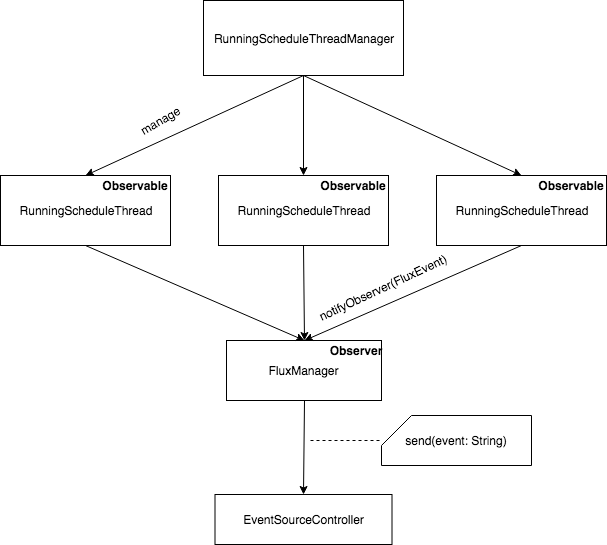
\includegraphics[width=0.8\linewidth]{schemas/flux_organisation.png}%
	\caption{Organisation des flux}
\end{figure}

En élément central, nous avons les RunningSchedulesThreads. Comme leur nom l'indique, c'est eux qui représentent l'exécution d'un Schedule actif. Ils sont gérés par un manager, qui permet de les activer ou désactiver ou simplement d'y avoir accès. Ils génèrent des événements selon les flux de leur Schedule et les transmettent au FluxManager via le patron de conception \textbf{Observer}. \newline
Le FluxManager est un Singleton dont les seules tâches sont de récupérer les Events générés par les différents RunningSchedulesThreads, construire le message de l'événement à envoyer (donc le type, l'url, les écrans concernés, etc) et de les transmettre aux écrans. Il utilise pour cela la méthode \textit{send(event: String)} fournie par l'EventSourceController.\newline
Comme précisé dans le chapitre Analyse et Architecture, un système de "bloc-minute" est utilisé pour organiser la diffusion de flux en créant un "bloc-horaire" qui est utilisé par les RunningSchedulesThreads pour déterminer quels flux doivent-ils envoyer et quand.

\subsubsection{Bloc-horaire}
La première implémentation (un peu naïve) que j'ai faites de ces horaires utilisait une simple liste de flux qui, si elle me permettait de vérifier le bon fonctionnement du programme n'offraient que peu de souplesse pour les différentes fonctionnalités à implémenter. Il a donc été choisi de représenter une plage d'affichage comme un ensemble de bloc et j'ai choisi comme valeur temporelle une minute afin de simplifier le processus et d'offrir une plus grande granularité à l'utilisateur.\newline
Concrètement, un "bloc-horaire" est une \textit{Map<Integer, Integer>} qui associe à chaque index de bloc l'id du flux programmé à cette heure-ci ou -1 afin de représenter une absence de flux. Il est construit à chaque fois qu'un Schedule est activé à partir de ses données puis fourni au RunningSchedulesThread associé. On peut voir dans la figure suivante la manière dont cet horaire est généré:

\lstinputlisting[caption=Création du bloc-horaire,language=Java]{code/timetable_creation.java}

On commence par récupérer les flux avec heure de début du Schedule concerné, puis on remplit l'horaire bloc par bloc en vérifiant à chaque fois si un flux est prévu pour le bloc courant. \newline
Ce système offre principalement deux avantages: 
\begin{itemize}
	\item Il est très facile de modifier le "bloc-horaire" d'un Schedule actif pour en modifier le comportement (changer de flux, en rajouter ou même en supprimer) sans devoir arrêter le programme.
	\item La reprise automatique de l'exécution des Schedules actifs est elle aussi très simple: le système inspecte la base de données au démarrage et si elle contient des RunningSchedules, il lance les threads associés.
\end{itemize}


 
\subsubsection{RunningScheduleThread}
C'est vraiment dans cette classe que la logique de "scheduling" est implémentée. Voici une version très simplifiée de sa méthode \textit{run()} mais qui garde la même logique fondamentale:

\lstinputlisting[caption=Eventsource Java,language=Java]{code/runninschedulethread_run.java}

Lorsqu'il débute, le thread récupère l'heure actuelle et vérifie qu'il est dans les bornes de la plage horaire. Si oui, il récupère l'indice du bloc courant puis commence son exécution. Dans le code ci-dessus ne figure pas toutes les opérations effectuées normalement mais il donne une assez bonne idée de son fonctionnement (l'extrait de code serait trop important sinon). Je préciserais quand même qu'on peut avoir une boucle infinie (lignes 26 à 48) dans le cas où aucun flux sans heure de début ne peut être casé. Ce problème est résolu mais pour des raison de clarté j'ai décidé d'enlever quelques parties de la fonction présentée. \newline
On peut résumer l'algorithme de choix de flux ainsi:


\begin{figure}[h]
	\centering	
	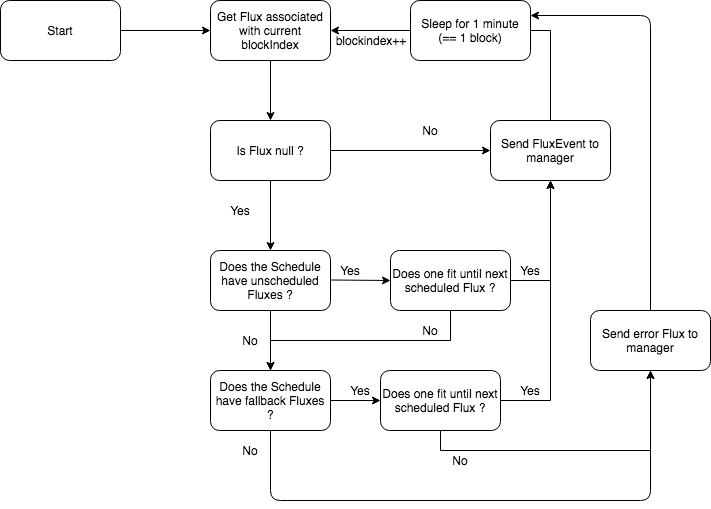
\includegraphics[width=0.8\linewidth]{schemas/runningschedulethread_algo.png}%
	\caption{Algorithme de scheduling des flux}
\end{figure}



\newpage
\subsubsection{FluxManager}

Le FluxManager est l'entité responsable de regrouper tout les Events générés par les Schedule pour les transmettre au contrôleur chargé de les envoyer aux écrans. C'est un Runnable Singleton qui est créé par injection de dépendance au démarrage de l'application et dont les contrôleurs ou autres objets peuvent obtenir une référence, par injection de dépendance à nouveau.
Pour représenter l'événement d'un flux, j'utilise un objet FluxEvent, qui est composé d'un flux et de la liste des adresses MAC des écrans concernés par cet événement. \newline
C'est également le FluxManager qui construit le contenu de l'Event qui sera envoyé aux écrans (voir Chapitre Analyse et Architecture, section Events).
Présenté ci-dessous, sa fonction \textit{run()} simplifiée:

\lstinputlisting[caption=FluxManager,language=Java]{code/fluxmanager_run.java}

La logique de cette classe est elle aussi plutôt simple; le FluxManager itère sur sa liste de FluxEvents et pour chacun d'entre eux il donne l'ordre au contrôleur d'envoyer un Event aux écrans. Dans le cas où il n'a pas de FluxEvent à traiter, il \textit{sleep} pendant quelques instants avant de recommencer la procédure.

\newpage
\subsection{Contrôleurs}

La plupart des contrôleurs de l'application servent uniquement à exécuter des opérations CRUD, mais certains offrent des fonctionnalités plus poussées qui sont décrites dans les sections suivantes.

\subsubsection{EventSource}

Lors des discussions préalables avec mon mentor, j'avais été prévenu que dans la version 2.7 de Play Java, les Eventources ne fonctionnaient pas car les informations de session étaient perdues lors d'un mapping. Travaillant avec la version 2.7.1 (sensée avoir résolu ce problème), je suis donc parti sur une implémentation en Java. J'ai d'abord pensé avoir réussi, car j'observais un comportement normal, mais en analysant de manière plus approfondie les échanges clients-serveurs lors d'une séance avec mon mentor, nous nous sommes aperçu que la connexion Eventsource était recréée toute les 3 secondes, quand le client essayait de se reconnecter au serveur. Il a donc été nécessaire de passer à une version en Scala.\newline
Ci-dessous une version simplifiée de l'ancien code Java:

\lstinputlisting[caption=Eventsource Java,language=Java]{code/eventsource.java}

L'idée de ce contrôleur était de mettre à jour une source à chaque fois qu'un Event devait être envoyé grâce au patron de conception \textit{Observer}. 
\newpage

Après un peu de recherche sur les différents moyen d'implémenter une utilisation des Eventsource en Scala, j'ai choisi une solution basée sur les Akka Actor. Elle semblait la plus simple et la plus adaptée à mon problème, car elle permet de représenter chaque écran par un acteur. \newline
Le contrôleur équivalent en Scala:

\lstinputlisting[caption=Eventsource Scala,language=Scala]{code/eventsource.scala}

On peut voir que ce contrôleur est au final très simple. Il offre deux actions principales: la possibilité pour un écran de s'enregistrer auprès du manager grâce à la méthode \textit{events()} et un moyen pour le système d'envoyer un Event aux écrans avec la méthode \textit{send(event: String)}. \newline
Il utilise pour ce faire un ActorSystem, construit à l'aide d'une sous-classe d'Actor, créée dans le cadre du projet. En voici l'implémentation:

\lstinputlisting[caption=Akka Actor Scala,language=Scala]{code/actors.scala}

\subsubsection{Ecrans}

C'est par ce contrôleur que passe les écrans souhaitant s'authentifier auprès du système et ainsi recevoir des flux. La logique du comportement étant décrite dans le chapitre \textbf{Protocole}, seul l'implémentation sera évoquée ici. \newline
Voici la version simplifiée de cette fonction:
\lstinputlisting[caption=Authentification des écrans,language=Java]{code/authenticate.java}

\subsubsection{Schedules}

Ce contrôleur permet d'activer et de désactiver des Schedules.

\paragraph{Activation}

\paragraph{Désactivation}


\subsubsection{Diffusers}

Ce contrôleur permet d'activer et de désactiver des Diffusers.

\paragraph{Activation}

\paragraph{Désactivation}


\newpage
\subsection{Vues}

\subsubsection{Affichage des flux}

L'affichage des Events reçus par les écrans se fait à l'aide d'une page HTML simple, qui défini les balises nécessaires à l'affichage des différents types de flux. A part un peu de CSS, rien d'autre ne s'y passe. En voici le body:

\lstinputlisting[caption=Eventsource HTML,language=HTML]{code/eventsource.html}

Il est couplé d'un script Javascript qui créé la connexion SSE avec le serveur et qui traite les Events qu'il reçoit par la suite. Selon le type de flux, il appelle des fonctions d'affichage différentes, qui agissent avec JQuery sur les balises présentées précédemment pour en modifier le contenu ou les cacher. Ci-dessous est présenté la fonction principale de ce script, avec l'analyse des Events reçus afin de déterminer le traitement adéquat:

\lstinputlisting[caption=Eventsource JS,language=java]{code/eventsource.js}


\subsubsection{Echange de données}

Pour échanger des informations entre le serveur et le client, j'ai choisi  d'utiliser les fonctionnalités offertes par Play!, donc avoir des entités représentant mes données (par exemple un Flux devient un FluxData) et les utiliser avec les templates Scala, Play permettant de facilement transférer des objets Java des contrôleurs aux vues. Ces templates sont des blocs de texte contenant du code Scala qui est par la suite compilé en HTML. Il devient alors facile de combiner cela à Bootstrap pour l'affichage ou l'envoi de données depuis le client.

Exemple d'entité:
\lstinputlisting[caption=UserData.java,language=java]{code/userdata.java}


\paragraph{Serveur -> client}

\lstinputlisting[caption=Exemple échange serveur-client,language=java]{code/server_to_client.java}

Ici, datautils.getAllTeams() renvoie une liste liste de \textbf{TeamData} qui sont récupérés et utilisés ensuite par le fichier html. On peut observer ici que l'intégration d'une boucle for avec une Table Bootstrap.

\paragraph{Client -> serveur}

\lstinputlisting[caption=Exemple échange client-serveur,language=java]{code/client_to_server.java}

Dans cet extrait de code, on a un exemple des fonctionnalités offertes par Play sous la forme de helpers servant à faciliter la création de formulaires Bootstrap. L'action effectuée par le bouton du formulaire est directement liée à la méthode de UserController.java. Il faut choisir comme valeur pour l'attribut name des balises input les noms des attributs correspondant dans le modèle correspondant (UserData en l'occurence).\newline
Le serveur est par la suite capable de reconstruire un objet du même type en récupérant le formulaire depuis la requête.
	
	
\newpage		
\section{Cas d'utilisation}
Les cas d'utilisation suivants sont regroupés par catégorie d'utilisateurs. Il y en a trois : les administrateurs, les chefs d'équipe (TeamAdmin) et les simples membres d'une équipe (TeamMember). Les admins ne sont associés à aucun écrans tandis que les deux autres sont restreints à certains écrans.
Toute action possible pour une catégorie l'est également pour celles en dessus. 

	\subsection{Administrateur:}
	L'admins peut effectuer toutes les actions et est le seul à pouvoir ajouter ou supprimer des écrans ou des utilisateurs au système. L'écran est allumé et connecté dans tous les cas suivants. \newline
		\begin{itemize}
		\item \textbf{Scénario 1:} Ajout d'un écran\newline
		\textbf{Déroulement:} L'admins rentre l'URL d'authentification des écrans dans le navigateur en spécifiant l'adresse MAC de l'écran comme paramètre de requête. Le serveur ne reconnait pas l'adresse MAC envoyée et renvoie donc un code servant à enregistrer l'écran dans le système. L'admins passe donc par le site pour ajouter l'écran en spécifiant entre autres son adresse MAC, son emplacement et le code fourni précédemment.\newline
		\textbf{Résultat:} L'écran sera maintenant reconnu par le serveur et correctement redirigé à la prochaine tentative.\newline
		\textbf{Erreurs potentielles:} Si la connexion est perdue entre l'écran et le backend à n'importe quel moment du scénario, les mêmes opérations seront effectuées à la re-connexion de l'écran (envoi du code). \newline
		
		\item \textbf{Scénario 2:} Mise à jour des infos d'un écran\newline
		\textbf{Pré-requis:} l'écran est déjà connu par le système.\newline
		\textbf{Déroulement:} L'admins se connecte au site et utilise l'interface fournie pour mettre à jour les infos souhaitées (nécessite potentiellement que l'écran ne soit pas actif).\newline
		\textbf{Résultat:} L'admins est informé du succès (ou de l'échec) de l'opération.\newline
		
		\item \textbf{Scénario 3:} Suppression d'un écran\newline
		\textbf{Pré-requis:} l'écran est déjà connu par le système.\newline
		\textbf{Déroulement:} L'admins se connecte au site et supprime l'écran du système en utilisant l'interface.\newline
		\textbf{Résultat:} L'admins est informé du succès (ou de l'échec) de l'opération et l'adresse MAC de l'écran est supprimée du système.\newline

		\item \textbf{Scénario 4:} Ajout d'un utilisateur\newline
		\textbf{Déroulement:} L'admins se connecte au site et ajoute l'utilisateur en utilisant l'interface fournie. Lors de l'ajout, il spécifie les écrans auxquels l'utilisateur pourra assigner des Schedules.\newline
		\textbf{Résultat:} L'admins est informé du succès (ou de l'échec) de l'opération et l'utilisateur est ajouté à la base de donnée.\newline

		\item \textbf{Scénario 5:} Modération: désactivation de Schedule\newline
		\textbf{Pré-requis:} Le Schedule est activé.\newline
		\textbf{Déroulement:} L'admins se connecte au site et va sur la page des Schedules. Dans la liste des actifs, il sélectionne celui qu'il veut désactiver et confirme son choix.\newline
		\textbf{Résultat:} L'admins est informé du succès (ou de l'échec) de l'opération et le Schedule est désactivé.\newline
		
		\item \textbf{Scénario 6:} Modération: désactivation de Diffuser\newline
		\textbf{Pré-requis:} Le Diffuser est activé.\newline
		\textbf{Déroulement:} L'admins se connecte au site et va sur la page des Diffusers. Dans la liste des actifs, il sélectionne celui qu'il veut désactiver et confirme son choix.\newline
		\textbf{Résultat:} L'admins est informé du succès (ou de l'échec) de l'opération, le Diffuser est désactivé et son flux est retiré des Schedules correspondants.\newline
		
		\item \textbf{Scénario 7:} Création d'une Team\newline
		\textbf{Déroulement:} L'admins se connecte au site et va sur la page des Teams. Il utilise l'interface fournie pour créer une nouvelle Team. Il doit spécifier à la création le nom de la Team et les écrans accessibles par ses membres. \newline
		\textbf{Résultat:} L'admins est informé du succès (ou de l'échec) de l'opération et la Team est créée et ajoutée en BD.\newline
		\textbf{Erreurs potentielles:} 
			\begin{itemize}
				\item Si le nom choisi pour la Team existe déjà, une erreur sera lancée et l'admins devra en choisir un autre.
			\end{itemize}
			
		\item \textbf{Scénario 8:} Modification d'une Team\newline
		\textbf{Pré-requis:} La Team existe.\newline
		\textbf{Déroulement:} L'admins se connecte au site et va sur la page des Teams. Il utilise la même interface que pour la création pour mettre à jour les infos souhaitées (nom, membres, admins).\newline
		\textbf{Résultat:} L'admins est informé du succès (ou de l'échec) de l'opération et la Team est modifiée.\newline
		\textbf{Erreurs potentielles:} 
			\begin{itemize}
				\item Si le nom choisi pour la Team existe déjà, une erreur sera lancée et l'admins devra en choisir un autre. \newline
			\end{itemize}
		
		\item \textbf{Scénario 9:} Suppression d'une Team\newline
		\textbf{Pré-requis:} La Team existe.\newline
		\textbf{Déroulement:} L'admins se connecte au site et va sur la page des Teams. Il sélectionne dans la liste celle qu'il souhaite supprimer et utilise l'interface fournie pour le faire. \newline
		\textbf{Résultat:} L'admins est informé du succès (ou de l'échec) de l'opération et la Team est supprimée. Les entités associés avec cette équipe sont également supprimées (Schedules et Diffuser). \newline

					
		\end{itemize}
		\newpage
	 
	\subsection{TeamAdmin:} 
	Un TeamAdmin ne peut ajouter d'écrans mais a la permission d'activer Schedules et Diffusers. \newline
		\begin{itemize}	
			\item \textbf{Scénario 1:} Activation d'un Schedule\newline
			\textbf{Pré-requis:} Le Schedule existe et les écrans choisis ne sont pas déjà assignés à un autre Schedule.\newline
			\textbf{Déroulement:} Le TeamAdmin se connecte au site et va sur la page des Schedules. Il choisit dans la liste affichée celui qu'il veut activer et utilise l'interface pour assigner des écrans ou groupes d'écrans à ce Schedule. Il peut ensuite activer son Schedule. \newline
			\textbf{Résultat:} Le TeamAdmin est informé du succès (ou de l'échec) de l'opération.\newline
			\textbf{Erreurs potentielles:} 
			\begin{itemize}
				\item Si le Schedule contient un flux restreint à un site et que l'on l'assigne à un écran sur un autre site, le système nous empêchera de le faire. Par contre, assigner un groupe d'écran avec un sous-ensemble de ce groupe d'un site différent sera possible (un flux de backup sera diffusé sur cet écran à la place).
				\item Si, parmi les écrans choisis, un ou plusieurs sont déjà assignés à un Schedule, le TeamAdmin en est prévenu et doit changer sa sélection. \newline
			\end{itemize}			
		
		\item \textbf{Scénario 2:} Activation d'un Diffuser\newline
			\textbf{Pré-requis:} Le Diffuser existe et les écrans choisis sont assignés à un Schedule.\newline
			\textbf{Déroulement:} Le TeamAdmin se connecte au site et va sur la page des Diffusers. Il choisit dans la liste affichée celui qu'il veut activer et utilise l'interface pour assigner des écrans ou groupes d'écrans à ce Diffuser. Il peut ensuite l'activer. \newline
			\textbf{Résultat:} Le TeamAdmin est informé du succès (ou de l'échec) de l'opération.\newline
			\textbf{Erreurs potentielles:} 
			\begin{itemize}
				\item L'heure de début prévue pour le flux du Diffuser est identique (ou à peine après) à l'heure de début d'un flux du Schedule. Il y a plusieurs manières de traiter ce cas: checker la durée du nouveau flux et reprendre l'exécution de l'ancien une fois fini, repousser un des deux flux (pas top je pense).\newline
			\end{itemize}			
			   
		\item \textbf{Scénario 3:} Création de groupe d'écrans\newline
			\textbf{Déroulement:} Le TeamAdmin se connecte au site et va sur la page des écrans. Il choisit les écrans (au moins 2) dans la liste pour son groupe et confirme son choix. (Les écrans peuvent appartenir à plusieurs groupes) \newline
			\textbf{Résultat:} Le TeamAdmin est informé du succès (ou de l'échec) de l'opération et le groupe est créé en BD.\newline	
			\textbf{Erreurs potentielles:} 
			\begin{itemize}
				\item Moins de 2 écrans sont choisis, le TeamAdmin est informé et doit choisir plus d'écrans.\newline
			\end{itemize}
			
		\item \textbf{Scénario 4:} Modification de groupe d'écrans\newline
			\textbf{Pré-requis:} Le groupe existe.\newline
			\textbf{Déroulement:} Le TeamAdmin se connecte au site et va sur la page des écrans/groupes. Il choisit dans la liste des groupes celui ou ceux qu'il désire modifier et utilise pour ce faire la même interface que pour la création de groupe. \newline
			\textbf{Résultat:} Le TeamAdmin est informé du succès (ou de l'échec) de l'opération et le groupe est modifié en BD.\newline	
			\textbf{Erreurs potentielles:} 
			\begin{itemize}
				\item Si le groupe est actuellement assigné à un RunningSchedule, la modification est empêchée et le TeamAdmin en est informé.
				\item Si le groupe modifié contient moins de deux écrans, la modification est empêchée et le TeamAdmin en est informé.\newline
			\end{itemize}
			
		\item \textbf{Scénario 5:} Suppression de groupe d'écrans\newline
			\textbf{Pré-requis:} Le groupe existe.\newline
			\textbf{Déroulement:} Le TeamAdmin se connecte au site et va sur la page des écrans/groupes. Il choisit dans la liste des groupes celui ou ceux qu'il désire supprimer et utilise l'interface fournie pour le faire. \newline
			\textbf{Résultat:} Le TeamAdmin est informé du succès (ou de l'échec) de l'opération et le groupe est supprimé en BD.\newline	
			\textbf{Erreurs potentielles:} 
			\begin{itemize}
				\item Si le groupe est actuellement assigné à un RunningSchedule, la suppression est empêchée et le TeamAdmin en est informé.\newline
			\end{itemize}
		
		\end{itemize}
		
		
	\subsection{TeamMember:} 
	Un TeamMember est assigné à une Team, qui elle à accès à des écrans, Schedules et Diffusers. Il peut créer et modifier des Schedules et Diffuser non-actifs mais ne peut pas les activer. Comme tous les autres types d'utilisateurs, il peut créer des flux. \newline
		\begin{itemize}
			\item \textbf{Scénario 1:} Création d'un flux\newline
			\textbf{Déroulement:} Le TeamMember se connecte au site et va sur la page des flux. Il entre les paramètres de son flux (à définir) \newline
			\textbf{Résultat:} Le TeamMember est informé du succès (ou de l'échec) de l'opération et le flux est ajouté à la liste des flux disponibles.\newline
			
			\item \textbf{Scénario 2:} Modification d'un flux\newline
			\textbf{Pré-requis:} Le flux existe.\newline
			\textbf{Déroulement:} Le TeamMember se connecte au site et va sur la page des flux. Il choisit le flux à modifier dans la liste et utilise la même interface que pour la création pour la mise à jour. \newline
			\textbf{Résultat:} Le TeamMember est informé du succès (ou de l'échec) de l'opération.\newline
			
			\item \textbf{Scénario 3:} Suppression d'un flux\newline
			\textbf{Pré-requis:} Le flux existe.\newline
			\textbf{Déroulement:} Le TeamMember se connecte au site et va sur la page des flux. Il choisit le flux à supprimer et confirme son choix.\newline
			\textbf{Résultat:} Le TeamMember est informé du succès (ou de l'échec) de l'opération et le flux est retiré de la liste des flux disponibles.\newline
			
			\item \textbf{Scénario 4:} Création d'un Schedule\newline
			\textbf{Pré-requis:} Des flux ont préalablement été créés.\newline
			\textbf{Déroulement:} Le TeamMember se connecte au site et va sur la page de création de Schedules. Il choisit les heures de début des flux en associant le flux voulu. Il peut encore spécifier le nom du Schedule ou un commentaire sur son utilité. Il confirme son choix. \newline
			\textbf{Résultat:} Le TeamMember est informé du succès (ou de l'échec) de l'opération et le Schedule est ajouté à la liste des Schedules disponibles.\newline
			\textbf{Erreurs potentielles:} Les heures de début de flux ne sont pas cohérentes (confirmation alors impossible). \newline
			
			\item \textbf{Scénario 5:} Modification d'un Schedule \newline
			\textbf{Pré-requis:} Le Schedule existe.\newline
			\textbf{Déroulement:} Le TeamMember se connecte au site et va sur la page des Schedules. Il choisit le Schedule à modifier dans la liste et utilise la même interface que pour la création pour la mise à jour. \newline
			\textbf{Résultat:} Le TeamMember est informé du succès (ou de l'échec) de l'opération.\newline
			\textbf{Erreurs potentielles:} Les heures de début des nouveaux flux ne sont pas cohérentes (confirmation alors impossible). \newline
			
			\item \textbf{Scénario 6:} Création d'un Diffuser\newline
			\textbf{Pré-requis:} Des flux ont préalablement été créés.\newline
			\textbf{Déroulement:} Le TeamMember se connecte au site et va sur la page de création de Diffuser. Il choisit les heures de début du flux voulu et précise sa durée de validité (en jours?, semaines?). Il peut encore spécifier le nom du Diffuser ou un commentaire sur son utilité. Il confirme son choix. \newline
			\textbf{Résultat:} Le TeamMember est informé du succès (ou de l'échec) de l'opération et le Diffuser est ajouté à la liste des Diffusers disponibles.\newline
			\textbf{Erreurs potentielles:} Les heures de début de flux ne sont pas cohérentes (confirmation alors impossible). \newline
			
			\item \textbf{Scénario 7:} Modification d'un Diffuser \newline
			\textbf{Pré-requis:} Le Diffuser existe.\newline
			\textbf{Déroulement:} Le TeamMember se connecte au site et va sur la page des Diffuser. Il choisit le Diffuser à modifier dans la liste et utilise la même interface que pour la création pour la mise à jour. \newline
			\textbf{Résultat:} Le TeamMember est informé du succès (ou de l'échec) de l'opération.\newline
			\textbf{Erreurs potentielles:} Les heures de début des nouveaux flux ne sont pas cohérentes (confirmation alors impossible). \newline

		\end{itemize}

\newpage		
\section{Mockups}
Les mockups suivant ne sont pas représentatifs de l'aspect final de l'application mais plutôt des fonctionnalités offertes.

\subsection{Utilisateurs}

	\begin{figure}[h]
		\centering
		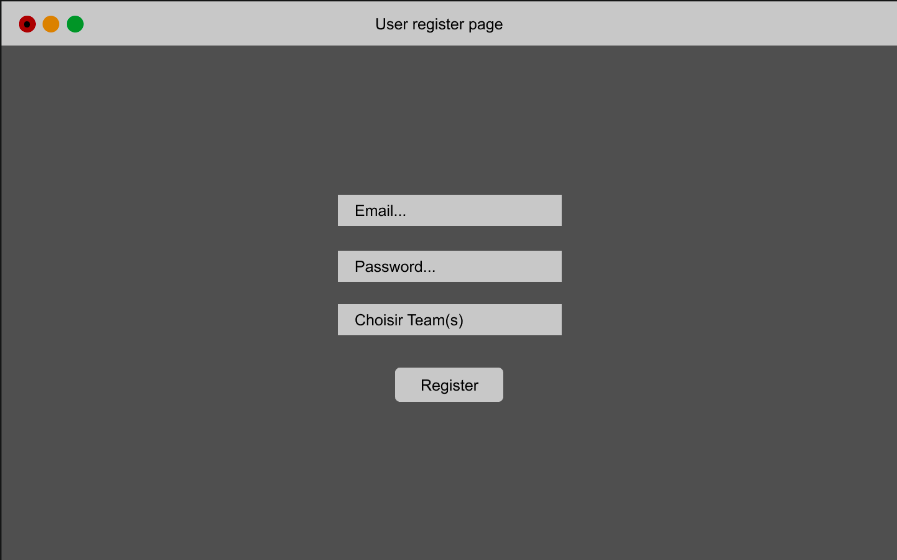
\includegraphics[scale=0.4]{mockup/m_user_register}
		\caption{Interface d'ajout de nouveaux utilisateurs}
		\label{fig:userRegister}
	\end{figure}
	
	Cette page en Figure ~\ref{fig:userRegister} sera uniquement accessible aux administrateurs (dans le cadre de mon TB en tout cas).
	
	\begin{figure}[h!]
		\centering
		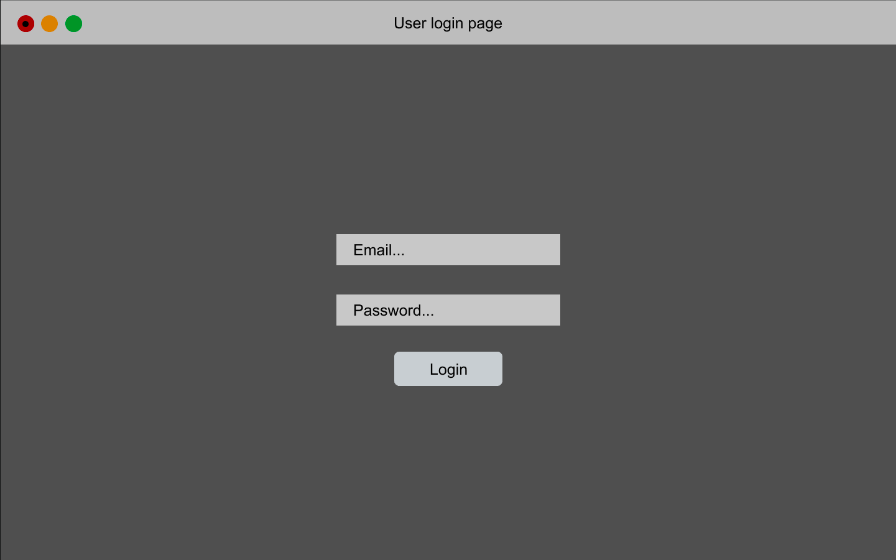
\includegraphics[scale=0.4]{mockup/m_user_login}
		\caption{Interface de connexion des utilisateurs}
		\label{fig:userLogin}
	\end{figure}
	
\newpage
\subsection{Ecrans}
	
	\begin{figure}[h]
		\centering
		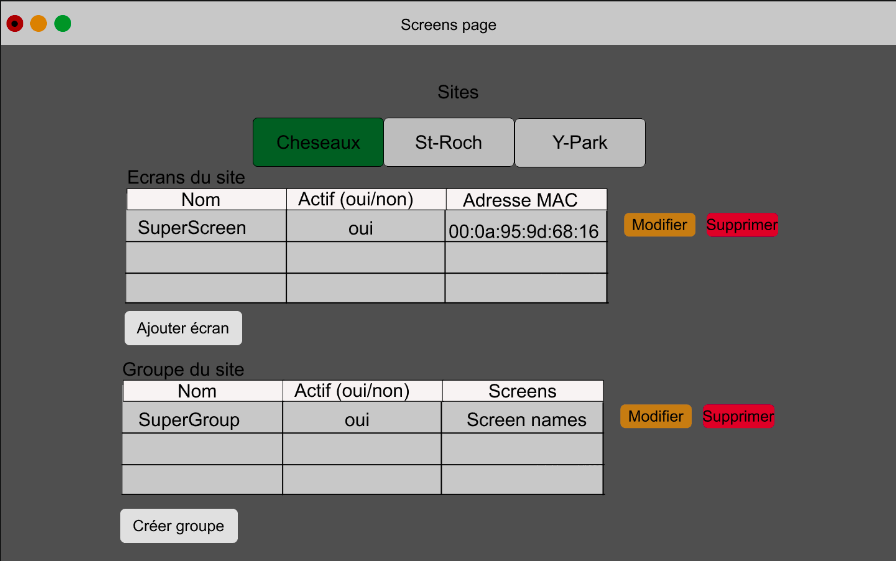
\includegraphics[scale=0.4]{mockup/m_screens_page}
		\caption{Page principale des écrans}
		\label{fig:screenPage}
	\end{figure}
	
	Cette page affiche les écrans accessibles par l'utilisateur actuel, regroupés par site. On a également accès aux groupes d'écrans. 
	
	\begin{figure}[h]
		\centering
		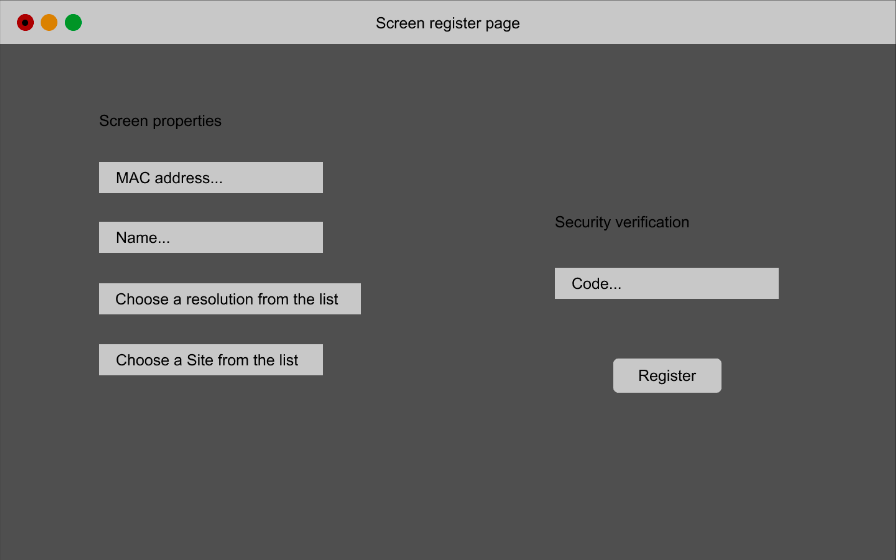
\includegraphics[scale=0.4]{mockup/m_screen_register}
		\caption{Interface d'ajout de nouvel écran}
		\label{fig:screenRegister}
	\end{figure}
	
	L'administrateur peut ajouter un nouvel écran au système par le biais de cette interface. Il doit préciser quelques paramètres et surtout donner le code fourni précédemment par le serveur.
	
	\begin{figure}[h]
		\centering
		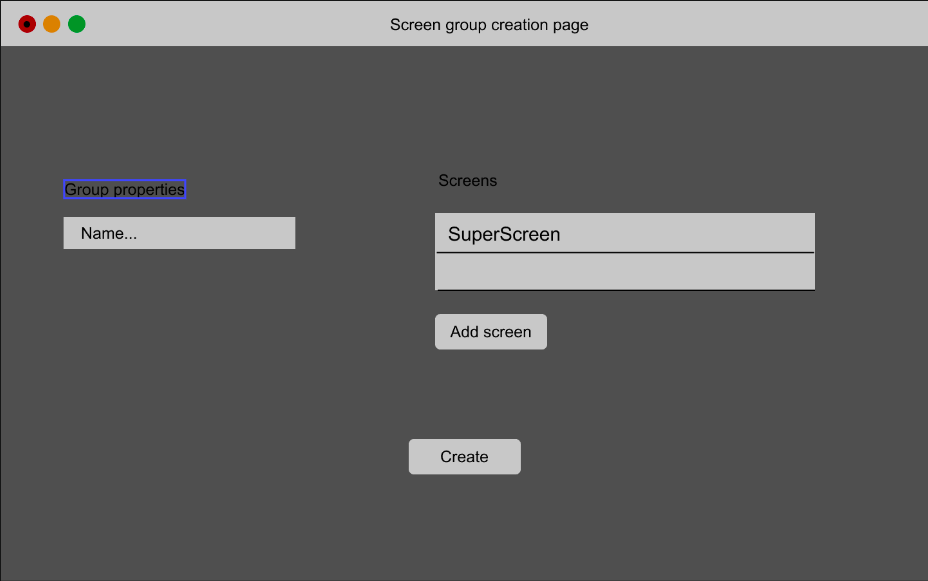
\includegraphics[scale=0.4]{mockup/m_group_creation}
		\caption{Interface d'ajout de nouveau groupe d'écran}
		\label{fig:groupCreation}
	\end{figure}
	
\newpage
\subsection{Teams}

	\begin{figure}[ht!]
		\centering
		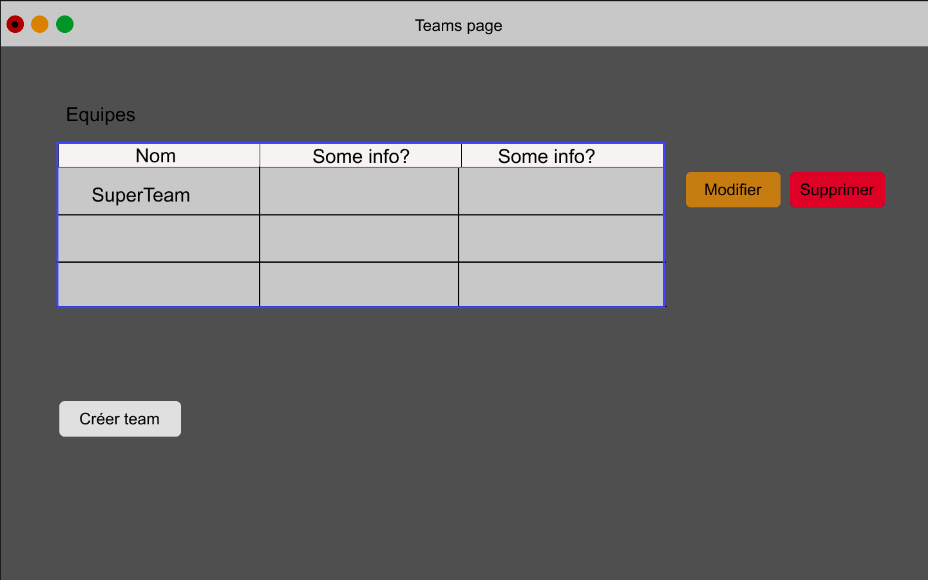
\includegraphics[scale=0.4]{mockup/m_teams_page}
		\caption{Page principale des teams}
		\label{fig:teamPage}
	\end{figure}
	
	\begin{figure}[h]
		\centering
		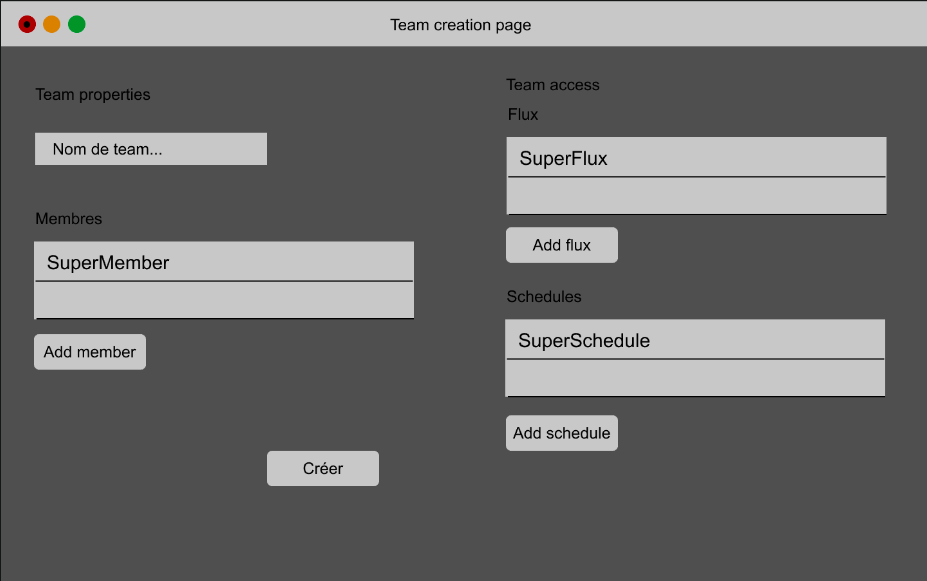
\includegraphics[scale=0.4]{mockup/m_team_creation}
		\caption{Interface de création de team}
		\label{fig:teamCreation}
	\end{figure}

\newpage	
\subsection{Flux}

	\begin{figure}[h]
		\centering
		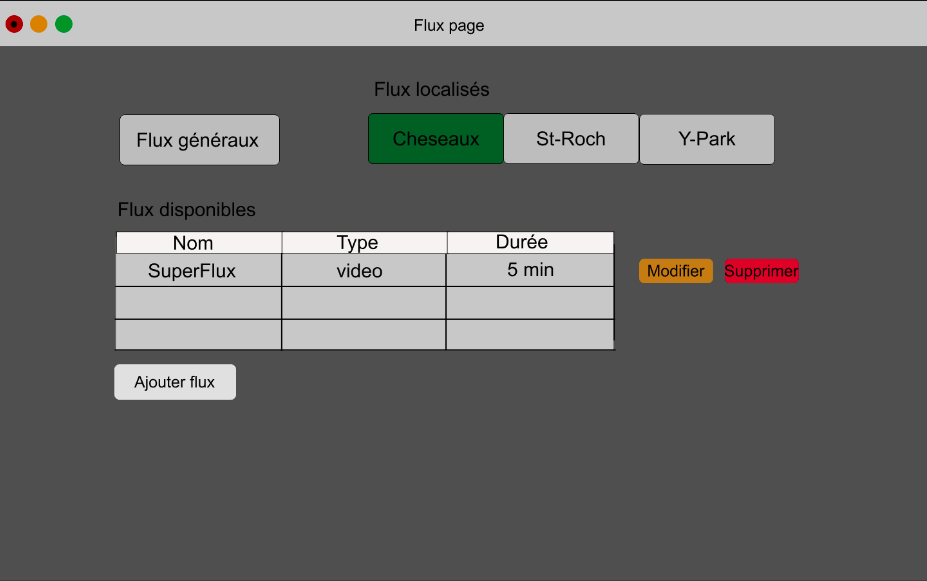
\includegraphics[scale=0.4]{mockup/m_flux_page}
		\caption{Page principale des flux}
		\label{fig:fluxPage}
	\end{figure}
	
	\begin{figure}[h]
		\centering
		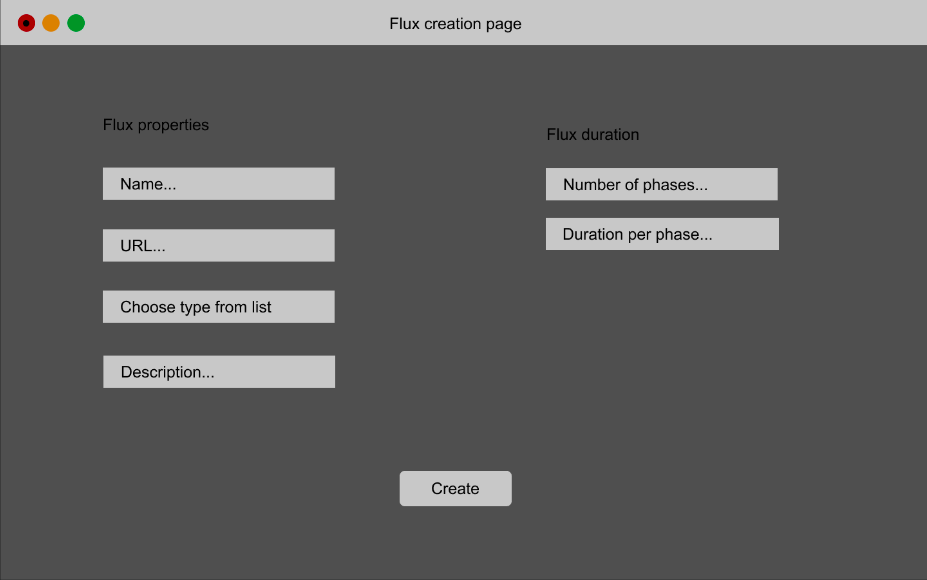
\includegraphics[scale=0.4]{mockup/m_flux_creation}
		\caption{Interface de création de flux}
		\label{fig:fluxCreation}
	\end{figure}
	
\newpage
\subsection{Schedules}

	\begin{figure}[h]
		\centering
		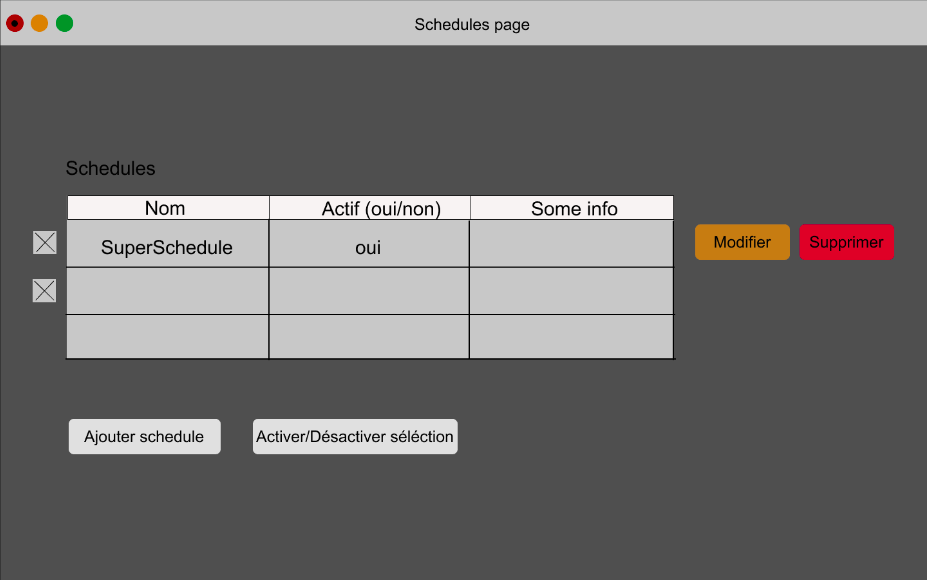
\includegraphics[scale=0.4]{mockup/m_schedules_page}
		\caption{Page principale des runningSchedules}
		\label{fig:schedulePage}
	\end{figure}
	
	\begin{figure}[h]
		\centering
		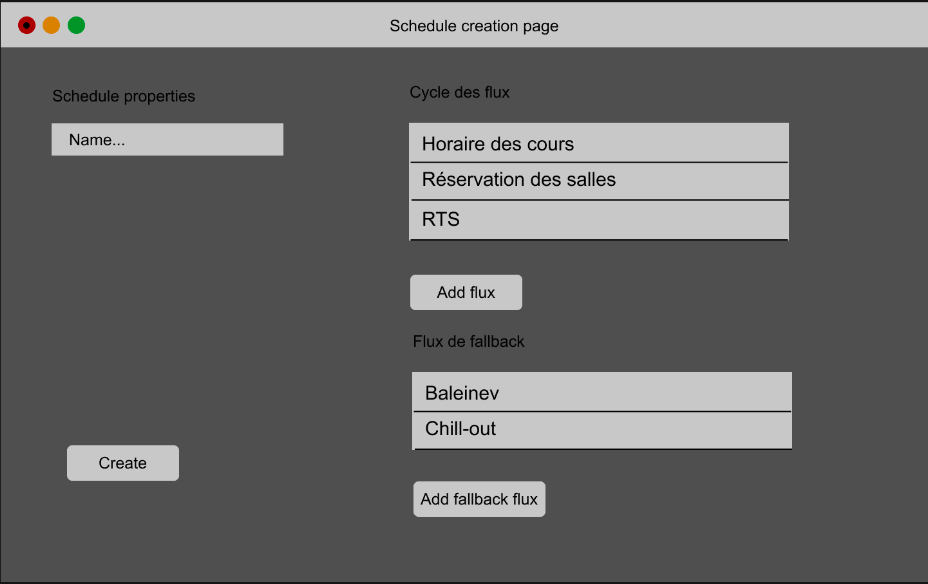
\includegraphics[scale=0.4]{mockup/m_schedule_creation}
		\caption{Interface de création de runningSchedule}
		\label{fig:scheduleCreation}
	\end{figure}
	
	On choisit les flux principaux qui vont constituer le cycle du Schedule. On peut également définir des flux de fallback qui prendront le relai si le flux actif n'a aucune information à afficher.

\newpage
\subsection{Diffusers}

	\begin{figure}[h]
		\centering
		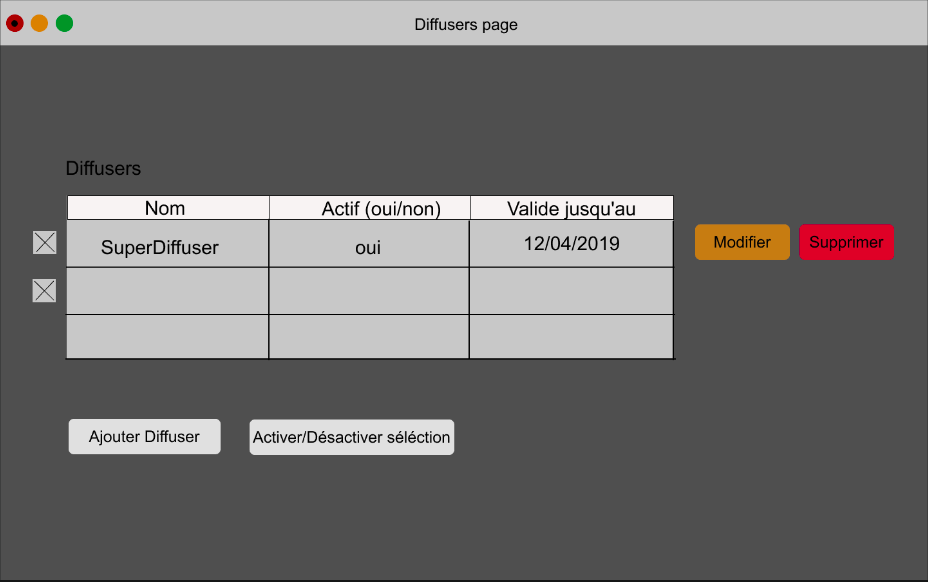
\includegraphics[scale=0.4]{mockup/m_diffusers_page}
		\caption{Page principale des diffusers}
		\label{fig:diffuserPage}
	\end{figure}
	
	\begin{figure}[h!]
		\centering
		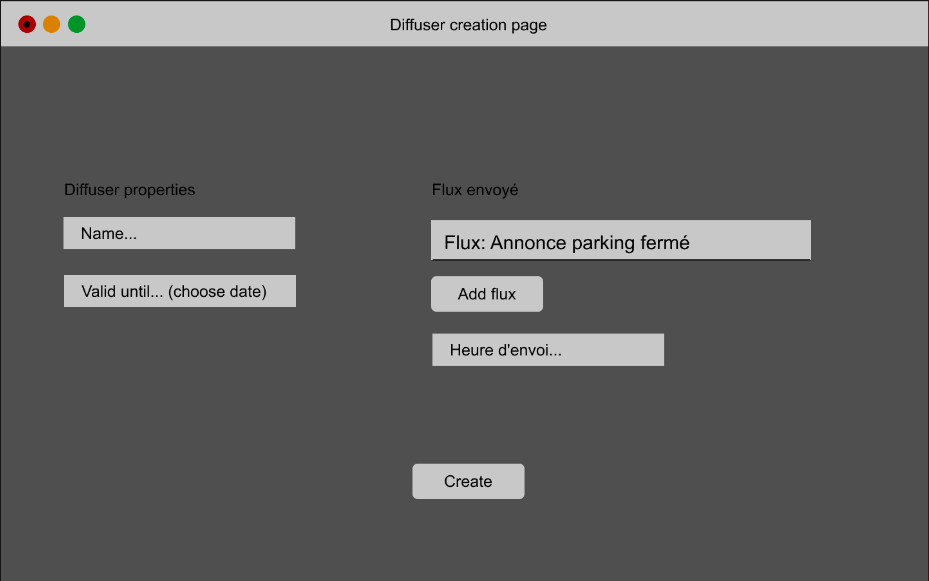
\includegraphics[scale=0.4]{mockup/m_diffuser_creation}
		\caption{Interface de création de diffuser}
		\label{fig:diffuserCreation}
	\end{figure}
	
	On spécifie la durée de validité du Diffuser en choisissant une date limite. 

	
\section{Tests}

\subsection{Tests JUnit}

\subsection{Tests fonctionnels}

\section{Remarques personnelles et commentaires}


\end{document}
















